\documentclass{beamer}
\usepackage{graphicx}
\usepackage{wrapfig}
\usepackage{hyperref}
\usepackage[norsk]{babel}

\title{Git-kurs}
\subtitle{Versjonkontroll med WebKom}
\institute{\url{https://github.com/kaprests/Gitkurs}}  % Don't want to bother, hack

\usetheme{metropolis}
%\usecolortheme{seagull}

\begin{document}
    \frame{
      \titlepage
    }

    \frame{
      \centering
      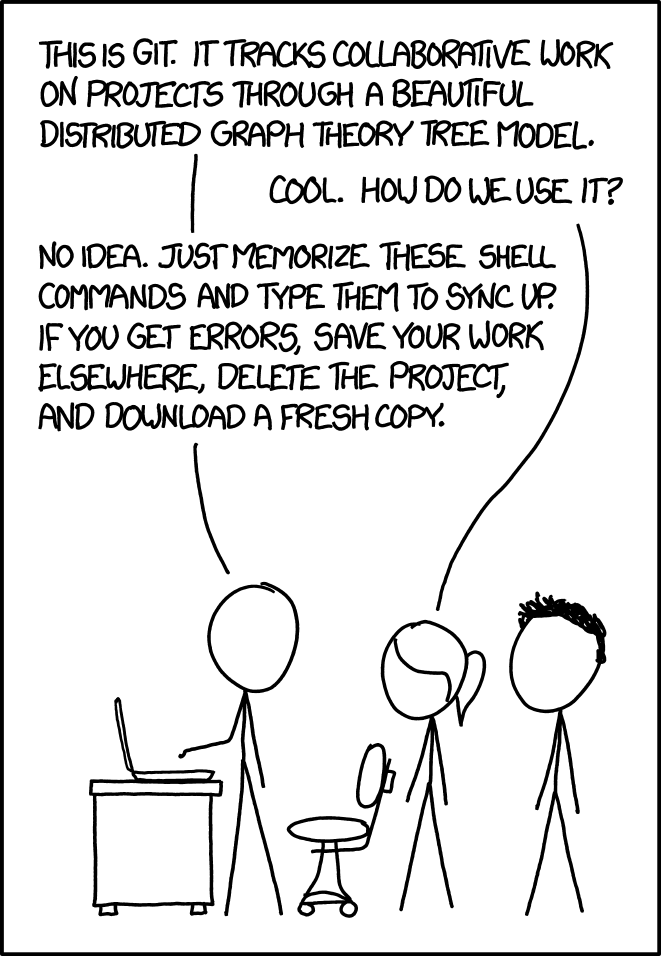
\includegraphics[width=0.5\textwidth]{xkcd_1.png}
    }

    \frame{
        \frametitle{Hva er git?}
        \begin{block}{GitHub}
            \begin{center}
                \huge Git $\neq$ GitHub!
            \end{center}    
        \end{block} 

        \begin{itemize}
            \item Git
                \begin{itemize}
                    \item Versjonkontrollprogram
                \end{itemize}
            \item GitHub
                \begin{itemize}
                    \item Vertstjeneste for git-repoer
                    \item Finnes flere alternativer (GitLab, Bitbucket etc.)
                \end{itemize}
        \end{itemize}
    }
    
    \frame{
      \frametitle{Hva er git?}

      \begin{itemize}
      \item Tar ``bilde'' av koden når du vil\\
      \item Gjør det enkelt å bla mellom ulike ``bilder''\\
      \item Man kan dele ``bildene'' med andre
      \end{itemize}
    }

    \frame{
        \frametitle{Terminologi}
        Noen viktige begreper
        \begin{wrapfigure}{r}{0.4\textwidth}
          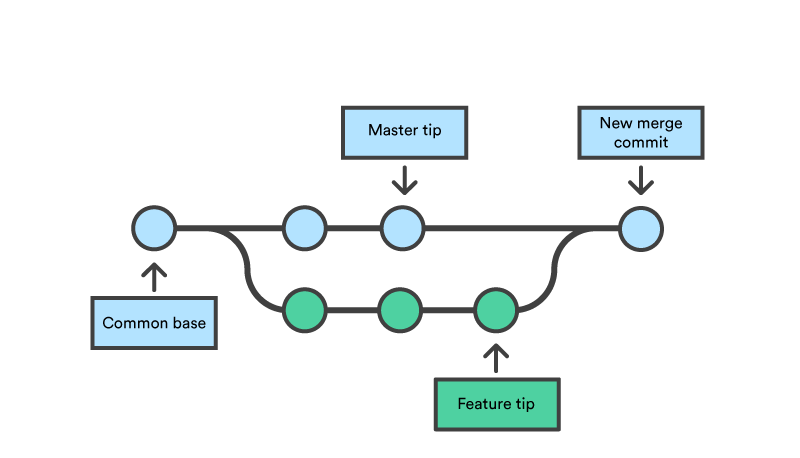
\includegraphics[width=0.5\textwidth]{branch.png}
        \end{wrapfigure}
        \begin{itemize}
            \item Commit
            \item Branch
            \item Repository
                \begin{itemize}
                    \item Lokalt/remote
                \end{itemize}
        \end{itemize}
        Om en forstår disse begrepene forstår en git.
    }

    \frame{
        \frametitle{Commit}
        Et slags ``snapshot'' av koden/prosjektet.
        \\
        \begin{wrapfigure}{r}{0.5\textwidth}
          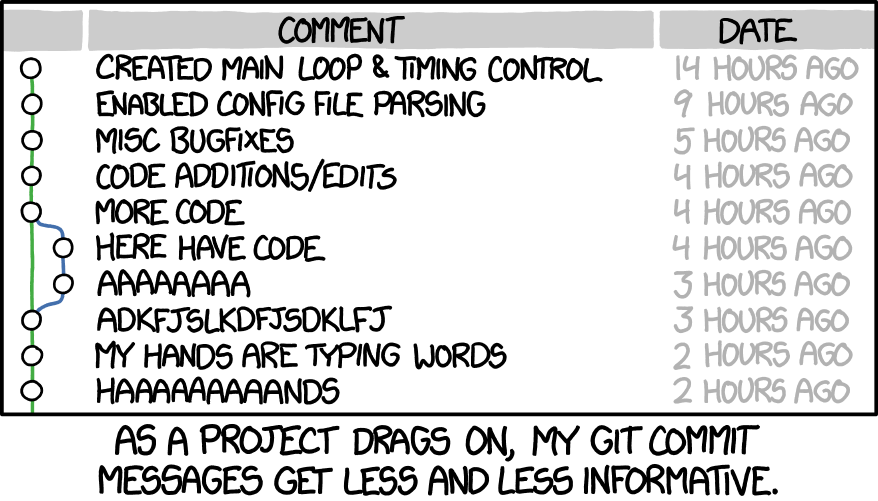
\includegraphics[width=0.5\textwidth]{xkcd_2.png}
        \end{wrapfigure}
        En commit består av:
        \begin{itemize}
            \item Endring fra forrige commit
            \item Forelder
            \item Hashkode
            \item Metadata
        \end{itemize}
        En oppretter commits på logiske/taktiske tidpunkter, f.eks. etter å ha fikset en bug 
        eller implementert en ny funksjon.\\\vspace{1em}
        En kan alltid returnere til en tidligere commit
    }

    \frame{
        \frametitle{Branch}
        Alle commits tilhører en branch\\
        Hovedbranch: master \\
        Head: referanse til nåverende branch\\
        Merging
        \begin{itemize}
            \item Sammenslåing av branches
            \item Mergekonflikter
        \end{itemize}
        For større endringer (mer enn en commit) oppretter en gjerne en egen branch som man commiter endringene 
        på, før en merger den inn i master.
    }

    \frame{
        \frametitle{Repository}
        Som regel prosjektmappen\\
        Inneholder:
        \begin{itemize}
            \item Alle filene du vil holde styr på og deres historikk
            \item Alle commits
        \end{itemize}
        Kan lagres på f.eks. GitHub
        \begin{itemize}
            \item cloning
            \item pull/push 
        \end{itemize}
    }

    \frame{
        \frametitle{Hvordan bruke git}
        Det finnes GUI
        \begin{itemize}
            \item ikke standard
        \end{itemize}
        Standard å bruke kommandolinjen\\
        Ulike IDE-er har ofte git-integrasjon og mulighet for å gjøre ting med GUI
    }

    \frame{
        \frametitle{Intro til kommandolinjen}
        Grunnleggende bruk, antar Linux eller Mac -terminal.\\
        For Windowsbrukere: git-bash\\
        Kommandoer:
        \begin{itemize}
            \item ls : list - printer innholdet i nåværende mappe
            \item cd \textless mappenavn \textgreater : change directory - bytt til mappe
            \begin{itemize}
                \item . betyr denne mappen .. betyr mappen over
                \item cd .. bytter altså til mappen over nåværende mappe
            \end{itemize}
            \item mkdir \textless nytt mappenavn \textgreater : Oppretter ny mappe
            \item cat \textless filnavn \textgreater : skriver ut innholdet til en fil
        \end{itemize}
        Dersom du kun bruker terminalen til git, så trenger du egentlig ikke å kunne mer enn de to første kommandoene, i tillegg til gitkommandoer da, såklart.
    }
    
    \frame{
        \frametitle{Oppgave: Bruke kommandolinjen}
        \begin{enumerate}
            \item Opprett en ny mappe med en eller flere filer
            \item Naviger til mappen i kommandolinjen med cd
            \item list innholdet i mappen med ls
            \item Opprett enda en ny mappe inne i mappen med mkdir
            \item Gå inn i den nye mappen med cd
            \item Gå tilbake til den første mappen med cd ..
        \end{enumerate}
    }

    \frame{
        \frametitle{Kommandoer}
        Oversikt over de viktigste kommandoene
        \begin{itemize}
            \item git init
            \item git add
            \item git commit
            \item git pull
            \item git push
            \item git branch
            \item git checkout
            \item git merge
            \item git clone
        \end{itemize}
    }

    \frame{
        \frametitle{Git arbeidsflyt - lokalt repo på din pc}
        \begin{enumerate}
            \item Gjør endringer
            \item Stage endringer med git add
            \item Lag commit med git commit
        \end{enumerate}
    }

    \frame{
        \frametitle{Git arbeidsflyt - repo med kun deg, med remote}
        \begin{enumerate}
            \item Gjør endringer
            \item Stage endringer med git add
            \item Lag commit med git commit
            \item Push endringer til origin (GitHub) med git push
        \end{enumerate}
    }

    \frame{
        \frametitle{Git arbeidsflyt - remote med flere bidragsytere, liten endring}
        \begin{enumerate}
            \item Gjør endringer
            \item Stage endringer med git add
            \item Lag commit med git commit
            \item Hent nyeste versjon fra origin med git pull
            \item Push endringer til origin (GitHub) med git push
        \end{enumerate}
    }

    \frame{
        \frametitle{Git arbeidsflyt - remote med flere bidragsytere, større endring}
        \begin{enumerate}
            \item Lag ny branch med git branch \textless navn på ny branch\textgreater
            \item Bytt til din nye branch med git checkout \textless navn på branch\textgreater
            \item Gjenta til endringen er klar
                \begin{enumerate}
                    \item Gjør endringer
                    \item Stage endringer med git add
                    \item Lag commit med git commit
                \end{enumerate}
            \item Bytt til master branch med git checkout master
            \item Hent nyeste versjon fra origin med git pull
            \item Merge din branch med endringer inn i master med git merge \textless navn på din branch\textgreater
            \item Push endringer til origin (GitHub) med git push
        \end{enumerate}
    }

    \frame{
        \frametitle{Oppgaver}
        Oppgave 1: Opprett et git-repositorry
        \begin{itemize}
            \item Lag prosjektmappe (ev. bruk noe du har fra før)
            \item Bytte til mappen/åpne en terminal i mappen
            \item git init
        \end{itemize}
    }

    \frame{
        \frametitle{Oppgaver}
        Oppgave 2: Commit noen endringer
        \begin{itemize}
            \item Gjør endringer (opprett/endre/slette file(er))
            \item Stage ønskede endringer (git add)
            \item Commit (git commit)
        \end{itemize}
        Gjenta dette noen ganger og skriv "git log" for å se commit-loggen.
    }

    \frame{
        \frametitle{Oppgaver}
        Oppgave 3: Få det på GitHub
        \begin{itemize}
            \item Opprett nytt, tomt repo på GitHub (uten README)
            \item Set remote
            \item Push til origin master
        \end{itemize}
        Når du har gjort dette kan fremtidige commits lastes opp til GitHub med bare "git push".\\-\\
        Får du til dette kan du nok til å bruke git med dine egne prosjekter!
    }

    \frame{
        \frametitle{Oppgaver}
        Oppgave 4: Samarbeid - prosjekt med flere bidragsytere
        \begin{itemize}
            \item ...
        \end{itemize}
    }

    \frame{
        \frametitle{Terminal cheat sheet (bash og mac)}
        \begin{itemize}
            \item bytte mappe: cd
                \begin{itemize}
                    \item cd ..  - (en mappe "opp")
                    \item cd Documents/gitkurs/ - (Bytt til mappen gitkurs)
                \end{itemize}
            \item mkdir \textless mappenavn\textgreater  - Opprett ny mappe
        \end{itemize}
    }

    \frame{
      \frametitle{Avsluttende tips}

      \textbf{GitHub Pro}\\
      Som student har du rett på GitHub Pro gjennom GitHub Education, dette er helt gratis!
      Se \url{https://education.github.com/pack}.

      \textbf{Grafisk tutorial på avansert bruk}
      \url{https://learngitbranching.js.org}
    }
\end{document}
